\documentclass[a4paper]{article}

\usepackage[utf8]{inputenc}
\usepackage[spanish]{babel}

\usepackage{fancyhdr,graphicx,listings,amsmath}
\usepackage[colorlinks=true,linkcolor=black,urlcolor=blue,bookmarksopen=true]{hyperref}

\newcommand{\materia}{[75.06 / 95.58] Organización de Datos}
\newcommand{\trabajo}{Trabajo Práctico 1: Análisis Exploratorio de Datos}
\newcommand{\trabajoheader}{TP1}
\newcommand{\cuatri}{2c2018}
\newcommand{\cuatrimestre}{Segundo cuatrimestre de 2018}
\newcommand{\grupo}{Grupo Datatouille}
\newcommand{\repo}{https://github.com/FdelMazo/7506-Datos/}
\newcommand{\kernel}{https://kaggle.com/datatouille2018/7506-TP1/}
\newcommand{\alumnos}{
    del Mazo, Federico & 100029 & delmazofederico@gmail.com\\
    Bojman, Camila & 101055 &  camiboj@gmail.com\\
    Hortas, Cecilia & 100687 & ceci.hortas@gmail.com\\
    Souto, Rodrigo & 97649 & rnsoutob@gmail.com\\
}
\newcommand{\curso}{Curso 01}
\newcommand{\docentes}{
    \item Argerich, Luis Argerich
    \item Golmar, Natalia
    \item Martinelli, Damina Ariel
    \item Ramos Mejia, Martín Gabriel
}

\hypersetup{
    pdftitle={\trabajo},
	pdfsubject={\materia},
	pdfauthor={\grupo},
}

\pagestyle{fancy}
\fancyhf{}
\fancyhead[L]{\materia}
\fancyhead[R]{\trabajoheader - \cuatri}
\renewcommand{\headrulewidth}{0.4pt}
\fancyfoot[C]{\thepage}
\renewcommand{\footrulewidth}{0.4pt}

\begin{document}
\pagenumbering{gobble}

\begin{titlepage}
	\hfill
\includegraphics[width=6cm]{fiuba.jpg}
    \begin{center}
    \vfill
    \Huge \textbf{\trabajo}
    \vskip2cm
    \Large \materia\\
    \cuatrimestre
    \vfill
    \begin{flushleft} 
    \grupo
    \end{flushleft}
    \begin{tabular}{|l|c|r|}
	\hline
	Alumno & Padrón & Mail\\
	\hline \hline
    \alumnos
	\hline
	\end{tabular}
    \begin{flushleft} 
    \url{\repo} \\
    \url{\kernel}
    \end{flushleft}
    \vskip1cm
    \end{center}
    \curso
    \begin{itemize}
        \docentes
    \end{itemize}
\end{titlepage}
\pagenumbering{roman}
\tableofcontents
\newpage
\pagenumbering{arabic}
\setcounter{page}{1}

\section{Introducción}

 Lorem ipsum dolor sit amet, consectetur adipiscing elit. Proin ultricies justo nisi, in ultrices lorem sollicitudin sed. Donec diam velit, aliquet et neque ac, tempus condimentum dolor. Maecenas scelerisque malesuada dignissim. Morbi sollicitudin est eu varius vestibulum. Duis sollicitudin non sapien quis iaculis. Quisque et luctus massa. In vitae odio vitae erat dapibus laoreet vitae in massa. Interdum et malesuada fames ac ante ipsum primis in faucibus. Nunc eu nunc tellus. Proin dignissim venenatis justo, vel rhoncus nibh commodo tincidunt. Suspendisse eleifend massa eget ligula viverra lacinia. Mauris egestas nisl a tincidunt rhoncus. 

\section{Análisis y desarrollo}

 Lorem ipsum dolor sit amet, consectetur adipiscing elit. Proin ultricies justo nisi, in ultrices lorem sollicitudin sed. Donec diam velit, aliquet et neque ac, tempus condimentum dolor. Maecenas scelerisque malesuada dignissim. Morbi sollicitudin est eu varius vestibulum. Duis sollicitudin non sapien quis iaculis. Quisque et luctus massa. In vitae odio vitae erat dapibus laoreet vitae in massa. Interdum et malesuada fames ac ante ipsum primis in faucibus. Nunc eu nunc tellus. Proin dignissim venenatis justo, vel rhoncus nibh commodo tincidunt. Suspendisse eleifend massa eget ligula viverra lacinia. Mauris egestas nisl a tincidunt rhoncus. 

La figura \ref{fig:radar_chart} es una gran figura.

\begin{figure}[!hb]
  \centering
    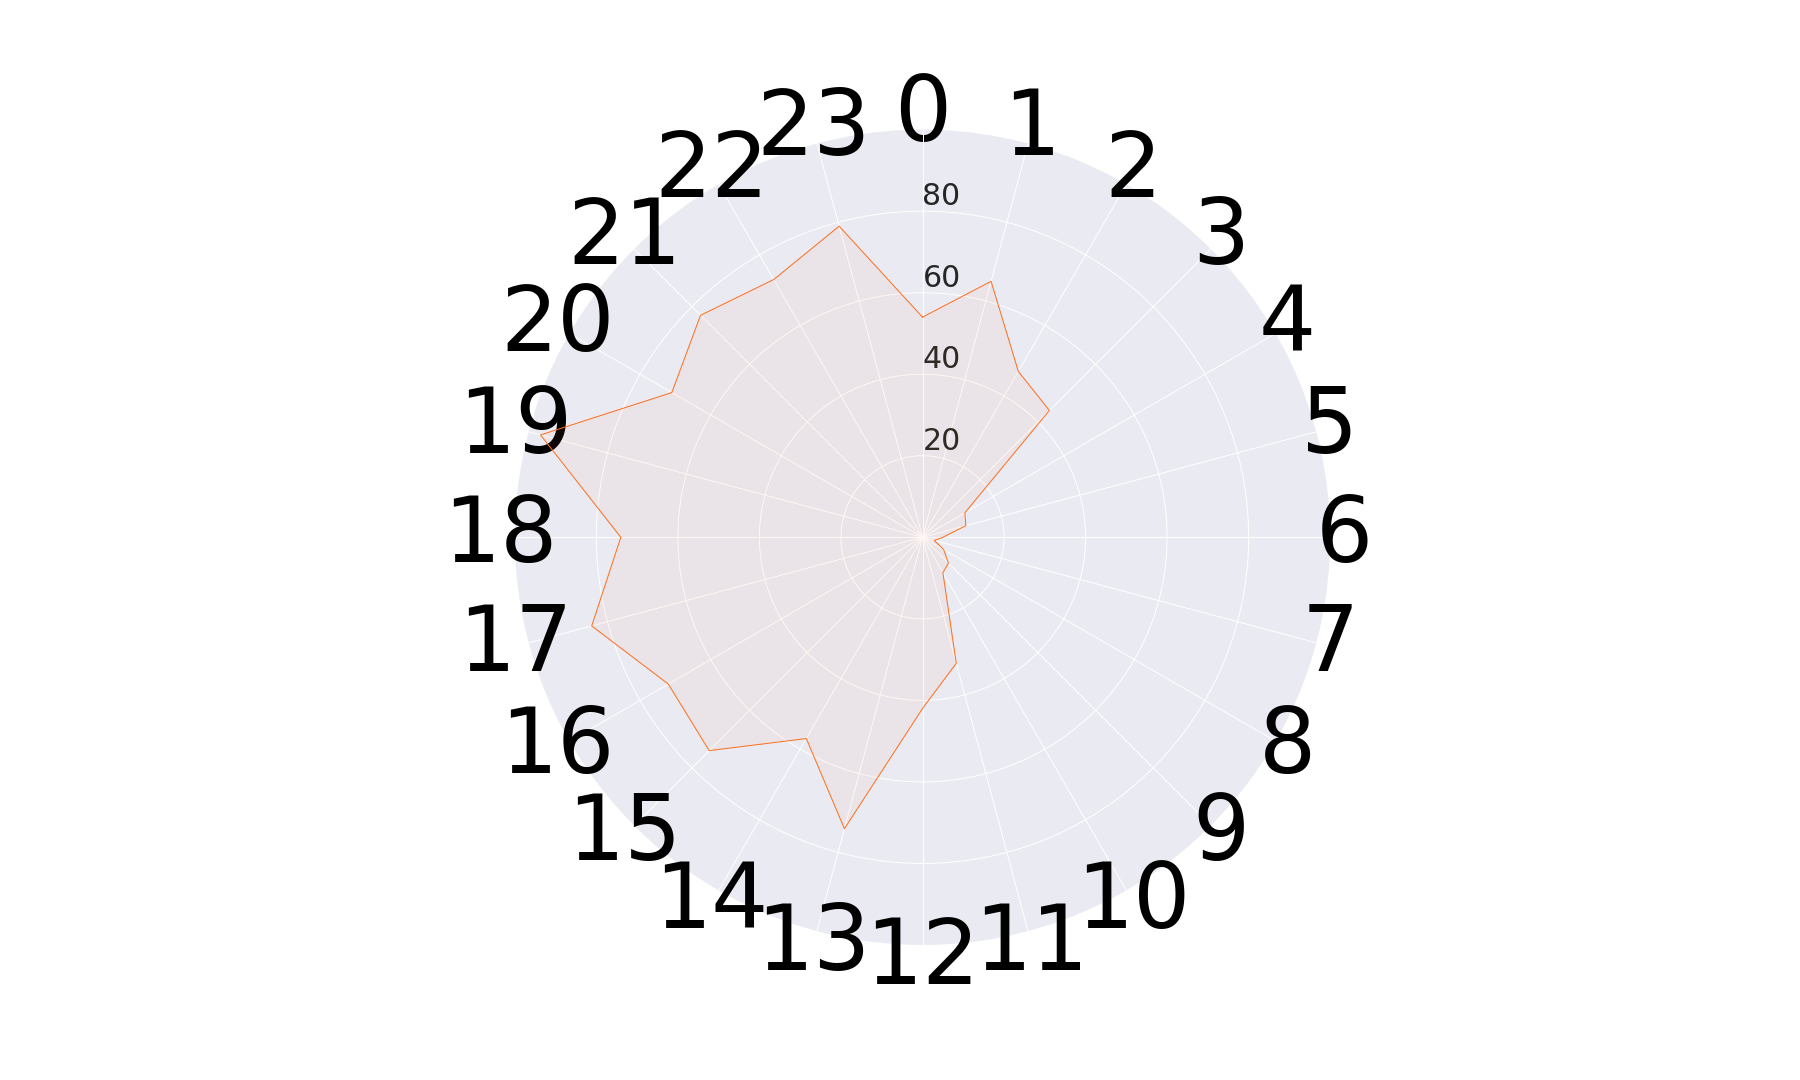
\includegraphics[width=0.5\textwidth]{figures/radar_chart.png}
  \caption{Radar chart}
  \label{fig:radar_chart}
\end{figure}

\section{Conclusiones, insights y aportes}

 Lorem ipsum dolor sit amet, consectetur adipiscing elit. Proin ultricies justo nisi, in ultrices lorem sollicitudin sed. Donec diam velit, aliquet et neque ac, tempus condimentum dolor. Maecenas scelerisque malesuada dignissim. Morbi sollicitudin est eu varius vestibulum. Duis sollicitudin non sapien quis iaculis. Quisque et luctus massa. In vitae odio vitae erat dapibus laoreet vitae in massa. Interdum et malesuada fames ac ante ipsum primis in faucibus. Nunc eu nunc tellus. Proin dignissim venenatis justo, vel rhoncus nibh commodo tincidunt. Suspendisse eleifend massa eget ligula viverra lacinia. Mauris egestas nisl a tincidunt rhoncus. 


\newpage
\appendix

\section{Ejecución}

El trabajo fue realizado en Anaconda \footnote{\url{https://anaconda.org/}}. Para poder replicar el trabajo, hay que también instalar las siguientes librerías adicionales:

\begin{itemize}
\item{Squarify \footnote{\url{https://github.com/laserson/squarify}}: Para los treemaps.}
\item{Geopandas \footnote{\url{http://geopandas.org/}}: Para poder graficar sobre mapas geográficos.}
\item{Wordcloud \footnote{\url{https://github.com/amueller/word_cloud/}}: Para poder visualizar los términos más buscados.}
\end{itemize}

Estos pueden ser instalados con los siguientes comandos: 

\begin{lstlisting}[language=sh]
pip install squarify
conda install -c conda-forge geopandas
conda install -c conda-forge wordcloud
\end{lstlisting}

\section{Datasets adicionales}

Los datasets adicionales y sus fuentes son:

\begin{itemize}
\item{Mapas de Brazil y Estados unidos: Sacados de Geonames \footnote{\url{http://www.geonames.org/}} }
\end{itemize}

\newpage

\end{document}
